\NeedsTeXFormat{LaTeX2e}
\documentclass[a4paper,11pt,final,DIV13,BCOR20mm,openbib,twoside,openany,onecolumn,pagesize,numbers=noenddot,bibliography=totoc,listof=totoc,index=totoc,
	headings=big,titlepage,toc=graduated,intoc,pdftex]{scrbook}
\usepackage[utf8]{inputenc}
\usepackage[ngerman]{babel}
\usepackage[T1]{fontenc}
\usepackage{lmodern}
\usepackage{url}
\usepackage{microtype}
\usepackage{xcolor}
\usepackage[pdftex]{graphicx}
\usepackage{amsmath}
\usepackage{amsthm}
\usepackage{pdfpages}
\usepackage{subfigure}
\usepackage{rotating}
\usepackage{nextpage}
\usepackage{float}
\usepackage[ruled,vlined,linesnumbered]{algorithm2e}
\usepackage{lscape}
\usepackage{csquotes}

\usepackage[absolute]{textpos}
\setlength{\TPHorizModule}{1mm}
\setlength{\TPVertModule}{\TPHorizModule}
\textblockorigin{0mm}{0mm}

\begingroup
\expandafter\expandafter\expandafter\endgroup
\expandafter\ifx\csname chapterformat\endcsname\relax\else
    \renewcommand*{\chapterformat}{
        \llap{
            \chapappifchapterprefix{\ }\thechapter\autodot\enskip
        }
    }
\fi

\renewcommand*{\othersectionlevelsformat}[1]{
    \llap{
        \csname the#1\endcsname\autodot\enskip
    }
}
\setlength{\unitlength}{1mm}
\newlength{\grafikdim}

\usepackage{listings}
\usepackage{color}
\renewcommand{\ttdefault}{pcr}
\definecolor{darkblue}{rgb}{0,0,.6}
\definecolor{darkred}{rgb}{.6,0,0}
\definecolor{darkgreen}{rgb}{0,.6,0}
\definecolor{red}{rgb}{.98,0,0}
\definecolor{mygreen}{rgb}{0,0.6,0}
\definecolor{mygray}{rgb}{0.5,0.5,0.5}
\definecolor{mymauve}{rgb}{0.58,0,0.82}

%\lstset{
 % %language=bash,
  %frame=none,
  %xleftmargin=0.7cm,
  %frame=tb
%}
\lstset{ %
  backgroundcolor=\color{white},   % choose the background color; you must add \usepackage{color} or \usepackage{xcolor}
  basicstyle=\footnotesize\ttfamily,            % the size of the fonts that are used for the code
  breakatwhitespace=false,         % sets if automatic breaks should only happen at whitespace
  breaklines=true,                 % sets automatic line breaking
  captionpos=b,
  columns=fixed,                   % sets the caption-position to bottom
  commentstyle=\color{mygreen},    % comment style
  deletekeywords={...},            % if you want to delete keywords from the given language
  escapeinside={\%*}{*)},          % if you want to add LaTeX within your code
  extendedchars=true,              % lets you use non-ASCII characters; for 8-bits encodings only, does not work with UTF-8
  frame=single,					   % adds a frame around the code
  keepspaces=true,                 % keeps spaces in text, useful for keeping indentation of code (possibly needs columns=flexible)
  keywordstyle=\color{blue},       % keyword style
  language=Prolog,
  literate=*{\#}{{\textcolor{blue}{\#}}}{1},
  otherkeywords={X,Y,tweety, pingu, woody, r1405, r1406, r1411, r1405B, program, external, not, kitchen, livingRoom},               % if you want to add more keywords to the set
  numbers=left,                    % where to put the line-numbers; possible values are (none, left, right)
  numbersep=5pt,                   % how far the line-numbers are from the code
  numberstyle=\tiny\color{mygray}, % the style that is used for the line-numbers
  rulecolor=\color{black},         % if not set, the frame-color may be changed on line-breaks within not-black text (e.g. comments (green here))
  showspaces=false,                % show spaces everywhere adding particular underscores; it overrides 'showstringspaces'
  showstringspaces=false,          % underline spaces within strings only
  showtabs=false,                  % show tabs within strings adding particular underscores
  stepnumber=1,                    % the step between two line-numbers. If it's 1, each line will be numbered
  stringstyle=\color{mymauve},     % string literal style
  tabsize=2,                       % sets default tabsize to 2 spaces
  title=\lstname,                  % show the filename of files included with \lstinputlisting; also try caption instead of title
  xleftmargin=2em,
  framexleftmargin=1.5em
  %linewidth=0.8\linewidth
}

\lstdefinestyle{keywordless}{
  backgroundcolor=\color{white},   % choose the background color; you must add \usepackage{color} or \usepackage{xcolor}
  basicstyle=\footnotesize\ttfamily,            % the size of the fonts that are used for the code
  breakatwhitespace=false,         % sets if automatic breaks should only happen at whitespace
  breaklines=true,                 % sets automatic line breaking
  captionpos=b,
  columns=fixed,                   % sets the caption-position to bottom
  commentstyle=\color{mygreen},    % comment style
  deletekeywords={...},            % if you want to delete keywords from the given language
  escapeinside={\%*}{*)},          % if you want to add LaTeX within your code
  extendedchars=true,              % lets you use non-ASCII characters; for 8-bits encodings only, does not work with UTF-8
  frame=single,					   % adds a frame around the code
  keepspaces=true,                 % keeps spaces in text, useful for keeping indentation of code (possibly needs columns=flexible)
  keywordstyle=\color{blue},       % keyword style
  language=Prolog,
  otherkeywords={},               % if you want to add more keywords to the set
  numbers=left,                    % where to put the line-numbers; possible values are (none, left, right)
  numbersep=5pt,                   % how far the line-numbers are from the code
  numberstyle=\tiny\color{mygray}, % the style that is used for the line-numbers
  rulecolor=\color{black},         % if not set, the frame-color may be changed on line-breaks within not-black text (e.g. comments (green here))
  showspaces=false,                % show spaces everywhere adding particular underscores; it overrides 'showstringspaces'
  showstringspaces=false,          % underline spaces within strings only
  showtabs=false,                  % show tabs within strings adding particular underscores
  stepnumber=1,                    % the step between two line-numbers. If it's 1, each line will be numbered
  stringstyle=\color{mymauve},     % string literal style
  tabsize=2,                       % sets default tabsize to 2 spaces
  title=\lstname,                  % show the filename of files included with \lstinputlisting; also try caption instead of title
  xleftmargin=2em,
  framexleftmargin=1.5em
}

\colorlet{punct}{red!60!black}

\lstdefinestyle{json}{
  backgroundcolor=\color{white},   % choose the background color; you must add \usepackage{color} or \usepackage{xcolor}
  basicstyle=\footnotesize\ttfamily,            % the size of the fonts that are used for the code
  breakatwhitespace=false,         % sets if automatic breaks should only happen at whitespace
  breaklines=true,                 % sets automatic line breaking
  captionpos=b,
  columns=fixed,                   % sets the caption-position to bottom
  commentstyle=\color{mygreen},    % comment style
  deletekeywords={...},            % if you want to delete keywords from the given language
  escapeinside={\%*}{*)},          % if you want to add LaTeX within your code
  extendedchars=true,              % lets you use non-ASCII characters; for 8-bits encodings only, does not work with UTF-8
  frame=single,					   % adds a frame around the code
  keepspaces=true,                 % keeps spaces in text, useful for keeping indentation of code (possibly needs columns=flexible)
  keywordstyle=\color{blue},       % keyword style
  language=Prolog,
  otherkeywords={},               % if you want to add more keywords to the set
  numbers=left,                    % where to put the line-numbers; possible values are (none, left, right)
  numbersep=5pt,                   % how far the line-numbers are from the code
  numberstyle=\tiny\color{mygray}, % the style that is used for the line-numbers
  rulecolor=\color{black},         % if not set, the frame-color may be changed on line-breaks within not-black text (e.g. comments (green here))
  showspaces=false,                % show spaces everywhere adding particular underscores; it overrides 'showstringspaces'
  showstringspaces=false,          % underline spaces within strings only
  showtabs=false,                  % show tabs within strings adding particular underscores
  stepnumber=1,                    % the step between two line-numbers. If it's 1, each line will be numbered
  stringstyle=\color{black},     % string literal style
  tabsize=2,                       % sets default tabsize to 2 spaces
  title=\lstname,                  % show the filename of files included with \lstinputlisting; also try caption instead of title
  xleftmargin=2em,
  framexleftmargin=1.5em,
   literate=
      {:}{{{\color{punct}{:}}}}{1}
      {,}{{{\color{punct}{,}}}}{1}
      {\{}{{{\color{blue}{\{}}}}{1}
      {\}}{{{\color{blue}{\}}}}}{1}
      {[}{{{\color{blue}{[}}}}{1}
      {]}{{{\color{blue}{]}}}}{1}
      {\}}{{{\color{blue}{\}}}}}{1}
      {\{}{{{\color{blue}{\{}}}}{1}
}

\lstdefinestyle{black}{
  backgroundcolor=\color{white},   % choose the background color; you must add \usepackage{color} or \usepackage{xcolor}
  basicstyle=\footnotesize\ttfamily,            % the size of the fonts that are used for the code
  breakatwhitespace=false,         % sets if automatic breaks should only happen at whitespace
  breaklines=true,                 % sets automatic line breaking
  captionpos=b,
  columns=fixed,                   % sets the caption-position to bottom
  commentstyle=\color{mygreen},    % comment style
  deletekeywords={...},            % if you want to delete keywords from the given language
  escapeinside={\%*}{*)},          % if you want to add LaTeX within your code
  extendedchars=true,              % lets you use non-ASCII characters; for 8-bits encodings only, does not work with UTF-8
  frame=single,					   % adds a frame around the code
  keepspaces=true,                 % keeps spaces in text, useful for keeping indentation of code (possibly needs columns=flexible)
  keywordstyle=\color{blue},       % keyword style
  language=Prolog,
  otherkeywords={},               % if you want to add more keywords to the set
  numbers=left,                    % where to put the line-numbers; possible values are (none, left, right)
  numbersep=5pt,                   % how far the line-numbers are from the code
  numberstyle=\tiny\color{mygray}, % the style that is used for the line-numbers
  rulecolor=\color{black},         % if not set, the frame-color may be changed on line-breaks within not-black text (e.g. comments (green here))
  showspaces=false,                % show spaces everywhere adding particular underscores; it overrides 'showstringspaces'
  showstringspaces=false,          % underline spaces within strings only
  showtabs=false,                  % show tabs within strings adding particular underscores
  stepnumber=1,                    % the step between two line-numbers. If it's 1, each line will be numbered
  stringstyle=\color{black},     % string literal style
  tabsize=2,                       % sets default tabsize to 2 spaces
  title=\lstname,                  % show the filename of files included with \lstinputlisting; also try caption instead of title
  xleftmargin=2em,
  framexleftmargin=1.5em,
}

\setcounter{secnumdepth}{2}
\setcounter{tocdepth}{2}
\setlength{\parskip}{\medskipamount}
%\setlength{\parindent}{0pt}
\usepackage{soul}

\makeindex
\usepackage{nomencl}
\providecommand{\printnomenclature}{\printglossary}
\providecommand{\makenomenclature}{\makeglossary}
\makenomenclature

\AfterFile{t1lmss.fd}{
  \DeclareFontShape{T1}{lmss}{b}{n}
  {<->ssub*lmss/bx/n}{}
}

\usepackage{textcomp}
\usepackage[charter]{mathdesign}
\usepackage{footmisc}

\DeclareSymbolFont{cmsy}{OMS}{cmsy}{m}{n}
\DeclareSymbolFontAlphabet{\mathcal}{cmsy}

\usepackage{setspace}
\usepackage{hyperref}
\onehalfspacing
\pagestyle{headings}

\newcommand*{\ORIGchapterheadendvskip}{}
\let\ORIGchapterheadendvskip=\chapterheadendvskip
\renewcommand*{\chapterheadendvskip}{
    {
        \setlength{\parskip}{0pt}
        \noindent\rule{.3\textwidth}{3pt}\rule[2.5pt]{.7\linewidth}{.5pt}\par
    }
    \vskip1.2em
}

\makeatletter
\providecommand{\toclevel@lstlisting}{0}
\makeatother

\addtokomafont{caption}{\small}
\setkomafont{captionlabel}{\sffamily\bfseries}
\setcapindent{1em}
\renewcommand \theparagraph {(\arabic{paragraph})}
\renewcommand*{\lstlistlistingname}{List of Listings}

\usepackage{booktabs}
\usepackage{pifont}

\setlength{\nomlabelwidth}{.20\hsize}
\renewcommand{\nomlabel}[1]{#1 \dotfill}

\hyphenation{name-space}

\usepackage[citestyle=numeric-comp, backend=biber, maxbibnames=10,
	natbib=true, block=ragged]{biblatex}
\usepackage{array}
\usepackage{bigstrut}

\addbibresource{bibtex.bib}

\graphicspath{{../images/}}

\newcolumntype{M}[1]{>{\centering\arraybackslash}m{#1}}

\usepackage[section]{placeins}

\begin{document}
\pagenumbering{gobble}
\begin{titlepage}
\newcommand{\Titel}[2][\textwidth]{\renewcommand{\baselinestretch}{1.0}\hfil
            \parbox{#1}{\huge\bfseries\centering #2}\hfil\par}
\renewcommand{\subtitle}[2][\textwidth]{\renewcommand{\baselinestretch}{1.0}\hfil
            \parbox{#1}{\LARGE\centering\mbox{}\llap{--~}#2\rlap{~--}}\hfil\par}
\newcommand{\addLine}[2][\textwidth]{\renewcommand{\baselinestretch}{1.0}\hfil
            \parbox{#1}{\large\centering #2}\hfil\par}


\begin{textblock}{40}(30,27)
 
\includegraphics[scale=0.7]{images/unilogo.pdf}
\end{textblock}

\begin{textblock}{40}(120,22)
 
\includegraphics[scale=0.3]{images/vs-logo-en.pdf}
\end{textblock}

\addLine{}
\vspace{0.2\textheight}

\Titel{Titel}

%\vspace{0.09\textheight}
\vspace{0.03\textheight}


\vspace{0.03\textheight}
\addLine{Master Thesis of}
\addLine{\LARGE ...}
\addLine{Student number:}
\addLine{\LARGE ...}
\addLine{submitted in the department}
\addLine{\LARGE Distributed Systems}
\vspace{0.1\textheight} 
\addLine{
  \begin{tabbing}
   Primary Reviewer: \quad ~\=  ~~~\:...\\
   Secondary Reviewer: \quad ~\= ...\\
   Advisor: \quad \> ...
  \end{tabbing}
}
\vspace{0.04\textheight} 
%\addLine{\today}
\addLine{July 4, 2017}
\vspace{0.04\textheight} 
\addLine{University of Kassel}
\addLine{Faculty of Electrical Engineering and Computer Science}
\addLine{Summer Semester 2017}
\end{titlepage}

%\cleartooddpage[\thispagestyle{empty}]
%\newpage
%\cleartooddpage[\thispagestyle{empty}]
%\thispagestyle{empty}

%\thispagestyle{empty}
%\cleardoublepage


\cleardoublepage
\chapter*{Affidavit}
\begin{Large}
	\textbf{Eidesstattliche Erklärung:}
\end{Large}

Ich versichere, dass ich die Arbeit selbstständig und ohne Benutzung anderer als der angegebenen Quellen und Hilfsmittel angefertigt habe und alle Ausführungen, die wörtlich oder sinngemäß übernommen wurden, als solche gekennzeichnet sind, sowie dass die Arbeit in gleicher oder ähnlicher Form noch keiner anderen Prüfungsbehörde vorgelegt wurde.

\vspace*{2cm}

\qquad Kassel, July 4, 2017 \hfill
\rule{0.45\textwidth}{0.4pt}

\cleardoublepage
\chapter*{Abstract}
\vfill
Text ...
\vfill


%\cleardoublepage
%\cleartooddpage[\thispagestyle{empty}]
\addtocontents{toc}{\protect\enlargethispage{2\normalbaselineskip}}
\tableofcontents
%\cleardoublepage
\thispagestyle{empty}
\cleartooddpage[\thispagestyle{empty}]
%\cleartoevenpage[\thispagestyle{empty}]

\pagenumbering{arabic}
\setcounter{page}{1}
\thispagestyle{empty}
\chapter{Introduction}
\label{sec:introduction}

\cleartooddpage[\thispagestyle{empty}]
%\cleartoevenpage[\thispagestyle{empty}]

\chapter{Definition Of Task}
\label{sec:taskdef}


\cleartooddpage[\thispagestyle{empty}]
%\cleartoevenpage[\thispagestyle{empty}]

\chapter{Foundations}
\label{sec:foundations}

\section{ROS – Robot Operating System}
\label{sec:ros}

Das Robot Operating System (ROS) ist ein Open Source Programmiergerüst (Framework)  zur Programmierung von Software für Roboter. ROS bietet zahlreiche Bibliotheken und Tools zum organisieren von komplexen und unterschiedlichen Aufgaben, um ein robustes Zugsamenspiel zwischen den verschiedenen Hardwarekomponenten einer oder mehrerer Roboterplattformen zu gewährleisten.  Im wesentlichen besteht ROS aus Treiber, die Daten von Sensoren wie Kameras, Laserscannern und GPS-Modulen auslesen, Algorithmen zum erstellen von Karten, Pfadplanung oder allgemeiner Navigation, der Infrastruktur, welche die Komponenten des Robotersystems miteinander verbindet und die Datenpakete zwischen den Prozessen verwaltet und Werkzeuge, zur Visualisierung des Roboters, der Aufnahme von Sensordaten und zur Fehleranalyse. 
Ein ROS-System besteht aus einzelnen Programmen, die in ROS nodes (Knoten) genannt werden. Die Programme kommunizieren untereinander über sogenannte edges (Kanten), welche die Datenströme darstellen. Ein Konten kann Datenströme senden, dann published er eine Topic, sodass ein anderer Knoten auf diese Topic subscriben, also diese Nachricht empfangen kann. Die Knoten und Kanten werden über einen Master überwacht, den roscore. 
Anleitungen für die Installation und Herangehensweise sind unter wiki.ros.org zu finden. Fragen werden durch die große Online-Community von Nutzern und Entwicklern beantwortet. 
Auf Internetseiten wie github.com werden auf Grundlage der ROS-Bibliothek vorprogrammierte oder fertige Programme geteilt, wodurch Programmieraufwand für neue Projekte reduziert werden kann, da oft auf diese bereits bestehende Programme aufgebaut, oder diese komplett übernommen werden. Daraus lässt sich der größte Vorteil von ROS ableiten, das Zeitersparnis.
ROS kann in jeder modernen Programmiersprache implementiert werden, jedoch wird es aktuell primär in Python, C++ und Lisp implementiert. Als Betriebssystem wird ein Unix-basiertes Betriebssystem vorausgesetzt. 
Im Fachbereich Verteilte Systeme der Universität Kassel existieren bereits viele ROS Applikationen. Da diese Arbeit in das bestehende ROS-System integriert werden soll, wird mit dieser Arbeit eine ROS-Applikation entwickelt. Entsprechend wurde das Betriebssystem Ubuntu 18.04 und die Programmiersprache C++ als Grundlage verwendet. 





\section{ConceptNet}
\label{sec:cn}

Conceptnet ist ein multilinguales semantisches Netzwerk, welches menschliches Allgemeinwissen in eine für Computer verständliche Sprache übersetzen soll. Netzwerke sind Datensätze,welche aus Begriffen (Knoten) und derer Beziehungen (Kanten) bestehen\cite{sowa1987semantic}. Bei semantischen Netzwerken bestehen die Kanten aus Wörtern, die eine Bedeutung der Beziehung zwischen zwei Knoten zuordnen. Semantische Netzwerke dienen in der Computerlinguistik als objektorientierte Wissensrepräsentationsmethode (WRM) und sind dem Bereich der künstlichen Intelligenz zuzuordnen\cite{helbig2013semantische}. 
Oft werden Netzwerke als Graphen dargestellt. 

\begin{figure}[h]

	\begin{center}
	
	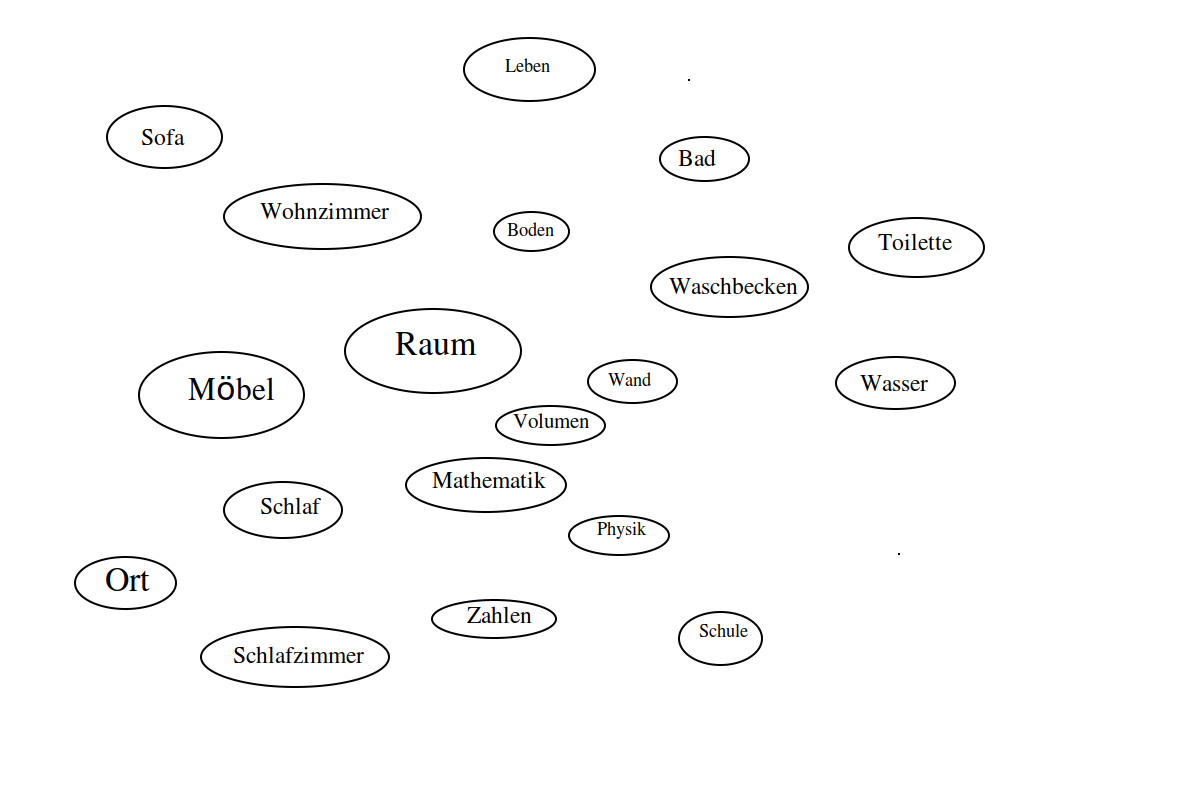
\includegraphics[width=18cm]{images/Netzwerk.png}
	
	\caption{Netzwerk}
	
	\label{netzwerk_Bild}
	
	\end{center}
	
	
\end{figure}

In Abbildung … ist ein semantisches Netzwerk dargestellt. Zu sehen ist, wie die Begriffe, zum Beispiel Wohnzimmer und Raum, zueinander in Beziehung stehen. Ein Wohnzimmer ist ein (IsA) Raum. IsA ist eine der 36 in Conceptnet Version 5.5 definierten Kernbeziehungen, die eine Deutung der Beziehung ermöglichen. Conceptnet Version 3 hat 26 Kernbeziehungen\cite{havasi2007conceptnet}. Weitere Beziehungen sind RelatedTo, welche einen Zusammenhang zweier Begriffe beschreibt, diese aber nicht genauer benennen kann und AtLocation, diese lässt auf einen Standort schließen. Ein Raum ist ein Ort, an dem sich Möbel befinden. 
In Conceptnet werden die Beziehungen in zwei Klassen eingeteilt, in symmetrische und asymmetrische Beziehungen. Zu den symmetrischen Beziehungen gehören beispielsweise RelatedTo, Synonym und Antonym. Hierbei handelt es sich um generellere Beziehungen, hingegen sind asymmetrische Beziehungen wie AtLocation, IsA, PartOf und UsedFor genauer definiert in Bezug auf ihre Deutungen. Eine weitere Eigenschaft des semantischen Netzwerkes ist das Kantengewicht, welches die Wichtigkeit der Beziehung abbildet. Ein Bett wird in Conceptnet mit einer Gewichtung von 10,9 in Beziehung zu Möbel gesetzt, eine Toilette mit einer Gewichtung von 0,17. Daraus lässt sich weiterer Kontext erschließen. 

\begin{figure}[h]
	
	\begin{center}
		
		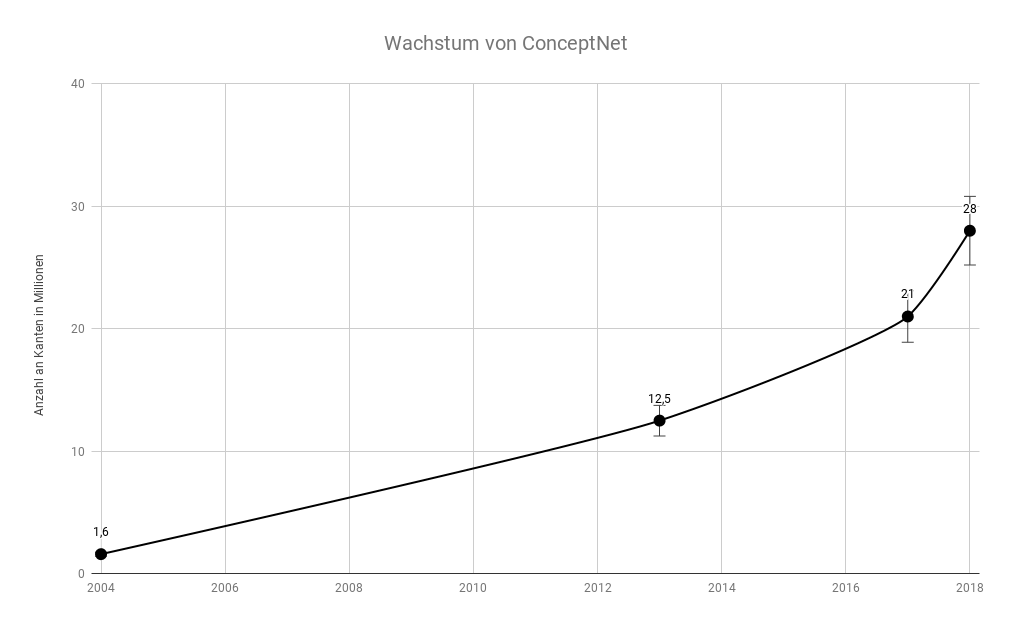
\includegraphics[width=16cm]{images/Wachstum_von_ConceptNet.png}
		
		\caption{Wachstum von Conceptnet}
		
		\label{wachstum_cn}
		
	\end{center}
	
	
\end{figure}


Abbildung ... zeigt das Wachstum von Conceptnet in Abhängigkeit der Anzahl der Beziehungen im zeitlichen Verlauf. Die Version 5.5 von Conceptnet weißt über 21 Millionen solcher Beziehungen auf und umfasst ach Millionen Begriffe. Da Conceptnet stetig weiterentwickelt wird, auf neue Ressourcen zugreift, vergrößert sich das Netzwerk und erzielt bessere Resultate. Bei der Version 5.6 wird die Anzahl der Beziehungen auf über 28 Millionen geschätzt, im Jahr 2004 waren es nur knapp zwei Millionen. 
Das Wissen von Conceptnet basiert ursprünglich auf Crowdsourcing Datensätzen wie wiktionary, DBpedia und Open-Mind-Common-Sense, auf Spielen wie verbosity und ndaya.jp und Expertenwissen von Wordnet, OpenCyc und JMDict. Ein neuer Ansatz ist Wissen von Word Embeddings, wie word2vec und GloVe, mit in Conceptnet zu integrieren. In \cite{speer2017conceptnet} werden unter dem Synonym ConceptNet Numberbatch bereits erste Erfolge nachgewiesen.

Zehn verschiedene Sprachen bilden den Kern von Conceptnet, in Summe sind über 300 Sprachen vertreten. Conceptnet hat sich in der Vergangenheit gegen andere semantische Netzwerke behauptet. Lediglich der Vergleich zu Cyc ist nicht genau zu validieren, da diese Plattform seit 2015 nicht mehr öffentlich zugänglich ist. Conceptnet hingegen ist ein Open Source Netzwerk und bietet die Möglichkeit über eine Web-API in eigene Anwendungen integriert zu werden. Wissenspakete im Json-Format können angefragt und für spezielle Aufgaben weiterverarbeitet werden. 
Die große Menge an Begriffen und der Wissensgehalt durch die Beziehungen von Conceptnet sind eine gute Voraussetzung als Wissensbasis für Künstliche Intelligenz und bieten eine Grundlage für diese Arbeit. 
\cite{liu2004conceptnet}
\cite{havasi2007conceptnet}
\cite{speer2013conceptnet}
\cite{speer2017conceptnet} 

\begin{align}
E &= mc^2
\end{align}






\cleartooddpage[\thispagestyle{empty}]
%\cleartoevenpage[\thispagestyle{empty}]

\chapter{Related Work}
\label{sec:relatedwork}


\cleartooddpage[\thispagestyle{empty}]
%\cleartoevenpage[\thispagestyle{empty}]

\chapter{Implementation}
\label{sec:implementation}

\section{Konzept}
\label{sec:Lösung}

Übergeordnet lässt sich die Aufgabe dieser Arbeit damit zusammenfassen, aus einem Bild Wissen zu ziehen, welches einen hohen Grad an Abstraktion beinhaltet. Da herkömmliche Neuronale Netzwerke alleine nicht für diese Aufgabe ausreichen, wird in dieser Arbeit der Ansatz untersucht, durch die Kombination aus Neuronalem Nerz und semantischem Netzwerk ein System zu schaffen und zu bewerten, welches aus einem Bild Informationen über z.B. die Räumlichkeit und Handlungsfelder, theoretisch aber über jegliches Thema, abstrahieren kann. 


\begin{figure}[h]
	
	\begin{center}
		
		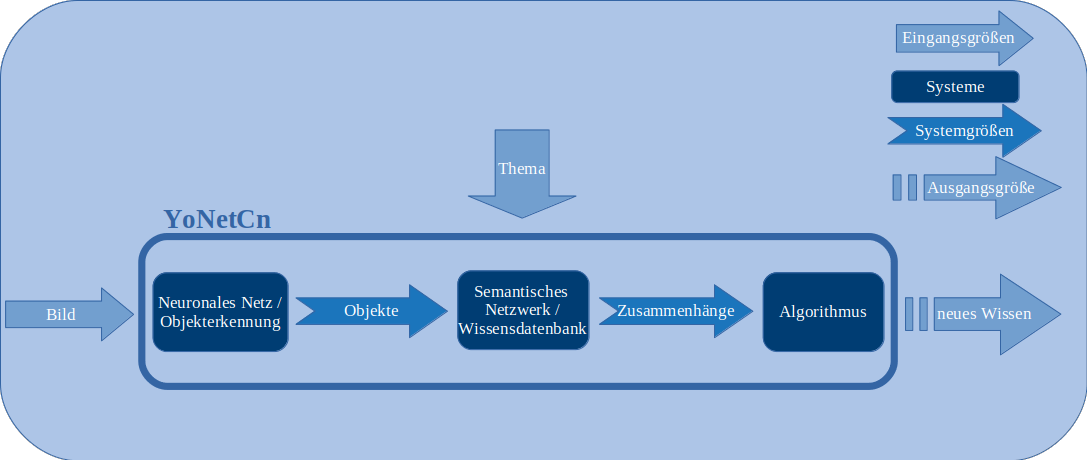
\includegraphics[width=14cm]{images/Masteridee.png}
		
		\caption{Aufbau System YoNetCn}
		
		\label{system_Bild}
		
	\end{center}
	
	
\end{figure}


In Abbildung \ref{system_Bild} ist das Konzept für dieses System, welches unter dem Namen YoNetCn zusammengefasst wird, dargestellt. Die primäre Eingangsgröße für YoNetCn ist ein Bild,in welchem durch ein Neuronales Netz Objekte erkannt werden. Die Objekte dienen zusammen mit der sekundären Eingangsgröße, einem Thema oder Themengebiet, einem Semantischen Netz als Eingangsgrößen. Ausgegeben werden vom semantischem Netz als Systemgröße die Zusammenhänge zwischen den Objekten und dem Thema. Ein Algorithmus bewertet und filtert diese Zusammenhänge und schließt daraus auf neues Wissen. Als Beispiel hierfür dient die Szenenerkennung. 



\begin{figure}[h]
	
	\begin{center}
		
		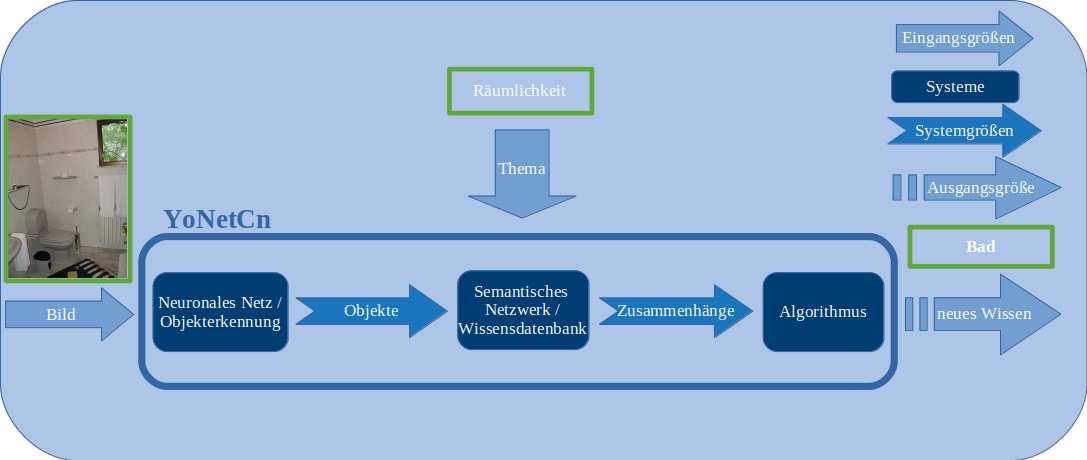
\includegraphics[width=14cm]{images/Masteridee_2.png}
		
		\caption{Szenenerkennung mit YoNetCn}
		
		\label{system_Bild2}
		
	\end{center}
	
	
\end{figure}


Abbildung \ref{system_Bild2} zeigt die Szenenerkennung mit YoNetCn am Beispiel eines Bildes von einem Bad. Wird zu diesem Bild das Thema Räumlichkeit als sekundäre Eingangsgröße eingegeben, so wird als Ausgabe Bad ausgegeben. Bei gleichem Bild, jedoch mit sekundärer Eingabe Tätigkeit, soll YoNetCn Adjektive wie duschen, auf Toilette gehen, oder Zähne putzen ausgeben. Theoretisch sind jegliche sekundären Eingangsgrößen möglich, jedoch wurde sich in dieser Arbeit auf die Themen Räumlichkeit und Tätigkeit beschränkt, da der zeitliche Rahmen dieser Arbeit ansonsten gesprengt werden würde und diese beiden Themengebiete als Nachweis für die grundsätzliche Durchführbarkeit der Aufgabenstellung ausreichen. 

\section{Umsetzung}
\label{sec:umsetzung}

In diesem Kapitel wird genauer auf die Umsetzung der drei Systemblöcke von YoNetCn eingegangen. Auch die Systemgrößen, Ein - und Ausgangsgrößen und Stellgrößen werden hier beschreiben. 



Auf Grundlage des konkreten Anwendungsbereiches von YoNetCn, der Servicerobotik, wurde als Stellgröße die Verarbeitungszeit und die Genauigkeit definiert. Ein Serviceroboter soll in Echtzeit erkennen können, welche Objekte sich in dem  Raum befinden, in welchem Raum er sich befindet und welche Handlungen mit den erkannten Objekten durchführbar sind. Da Echtzeit je nach Anwendungsbereich unterschiedlich ausgelegt wird, müssten für diesen Anwendungsfall genauere Untersuchungen für eine angemessene Reaktionszeit des Roboters durchgeführt werden, was jedoch nicht Umfang dieser Arbeit ist. Für YoNetCn wurde ein Wert von kleiner 10 Sekunden für die Reaktionszeit definiert, der Einfluss der Auslegung von YoNetCn auf die Reaktionszeit wird im Kapitel Evaluation genauer ermittelt. 

Die Genauigkeit von YoNetCn wird am Beispiel der Räumlichkeit genauer untersucht und es werden verschiedene Stell- und Störgrößen, deren Einfluss auf die Genauigkeit herausgearbeitet.
Als Beispiel hat ein großes Neuronales Netz, welches sehr viele Objekte erkennt, einen positiven Einfluss auf die Genauigkeit, jedoch wird dadurch die Verarbeitungszeit negativ beeinflusst, da größere Netze mehr Rechenoperationen als kleine benötigen. Entsprechend gilt es eine Balance zwischen den beiden Stellgrößen zu finden. 
Semantische Netzwerke basieren auf Sprache. Da Sprache mehrdeutig sein kann und unter Umständen zu Missverständnissen führt, allgemein nicht immer klar definiert ist im Vergleich zur Informatik und Mathematik, wird auch das Zusammenspiel zwischen dem Neuronalen Netz und dem Semantischen Netz untersucht und entsprechende Störgrößen herausgearbeitet. 


Da YoNetCn speziell für die Servicerobotik entwickelt wurde, besteht der Anspruch einer Einbindung in ein verteiltes System. Darunter ist zu verstehen, dass mehrere Roboter auf die Funktion von YoNetCn zugreifen können, ebenso die Ergebnisse zentral zugänglich sind. Die Vision, welche hinter diesem Anspruch steht, ist, dass in einer Umgebung, zum Beispiel ein Altenheim, mehrere Roboter mit unterschiedlichen Fähigkeiten eingesetzt werden können. Einer dieser Roboter hat eine Kamera und kann Bilder empfangen und diese an YoNetCn weiterleiten. Aus den Bildern werden Aufgaben abgeleitet, wie z.B. einen Kaffee kochen, oder das Geschirr aus dem Büro holen und dieses in der Küche in die Spülmaschine einräumen. Der Roboter mit der Kamera hat jedoch keinen Greifarm, ein andere wiederum schon. Die Aufgaben werden zentral gesteuert und an die Expertenroboter, welche entsprechende Aufgaben bewältigen können, weitergeleitet. So entsteht eine Kollaboration zwischen den Robotern. 

Auch zwischen den Robotern und den Menschen in der Umgebung, soll ein Austausch stattfinden. So erkennt ein Roboter Beispielsweise eine schmutzige, leere Kaffeetasse im Büro. Diese Information mit dem Wissen, dass in der Küche eine Kaffeemaschine steht, ermöglicht es, die Aufgabe des Kaffeekochens anzubieten. Über eine App auf dem Smartphone werden die entsprechenden Service angezeigt und können vom Menschen ausgewählt oder priorisiert werden. 

Ergänzend zur definierten Aufgabe dieser Arbeit wird daher eine Schnittstelle zum Menschen entwickelt. 

\begin{figure}[h]
	
	\begin{center}
		
		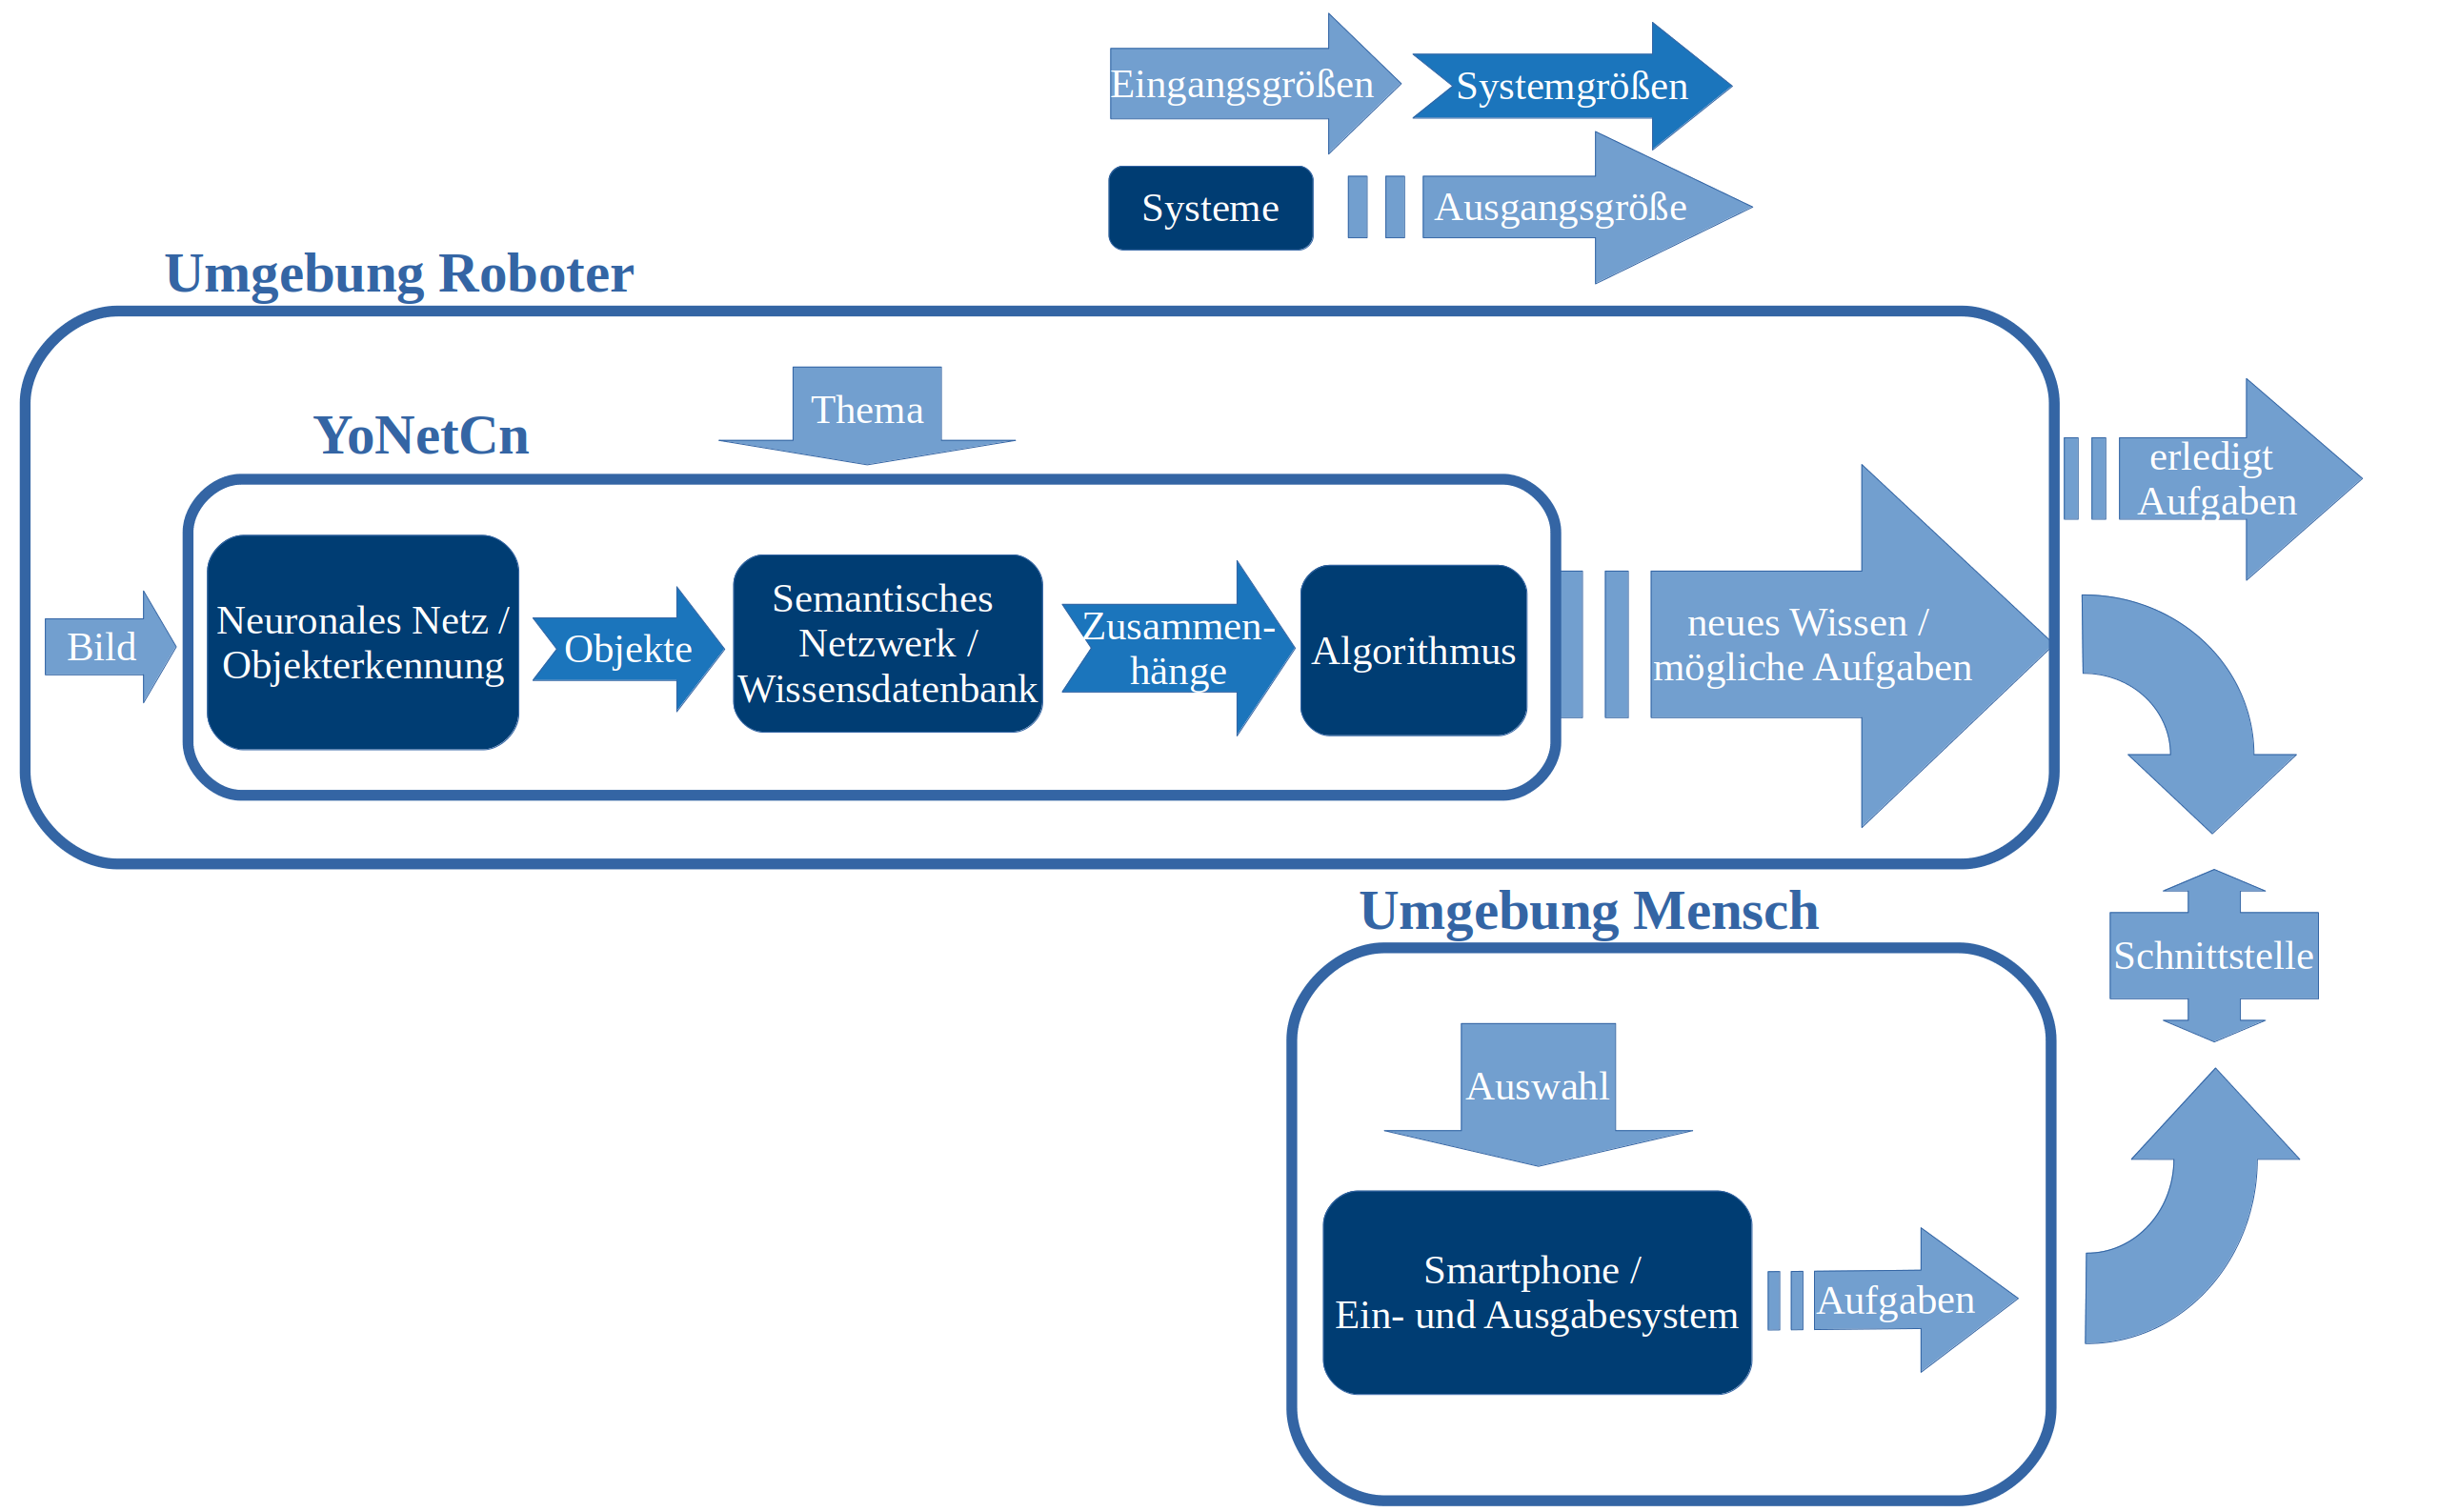
\includegraphics[width=16cm]{images/Masteridee_3.png}
		
		\caption{Roboter Mensch System}
		
		\label{Roboter_Mensch_System}
		
	\end{center}
	
	
\end{figure}


Abbildung \ref{Roboter_Mensch_System} zeigt die erweiterte Aufgabenstellung, welche eine Schnittstelle zwischen der Umgebung Roboter und der Umgebung Mensch beinhaltet. 
Über die Rückmeldung durch den Menschen, könnte noch eine Lernfunktion für die Roboterumgebung integriert werden, sodass beispielsweise Aufgaben die öfters ausgewählt wurden, von YoNetCn bevorzugt angeboten werden. Auch wäre es denkbar dem Menschen nicht nur eine Auswahl von Aufgaben anzubieten, sondern, dass dieser neue Aufgaben definiert oder sogar den Robotern Aufgaben beibringt. 
Die Umsetzung der angebotenen Aufgaben ist nicht Teil dieser Arbeit, es werden lediglich potenzielle Aufgaben von YoNetCn ausgegeben und der Umgebung Mensch mitgeteilt. 









Basieren auf den Vorgaben der Aufgabenbeschreibung, sind ROS und C++ als Software und Programmiersprache vorgegeben. Auf dem Rechner ist Ubuntu 18.04 als Betriebssystem installiert. Zunächst ist die aktuelle Version von ROS, ROS Melodic Morenia zu installieren. Dafür kann der Anleitung auf der wiki.ros.org Webseite gefolgt werden. 
ROS Melodic Morenia enthält das Paket OpenNi2launch, welches Bilder von einer über USB verbundenen Kamera als Ros Topic veröffentlicht. Da auch die in dieser Abreit verwendete Asus Kamera von OpenNi2 unterstützt wird, wurde dieses Paket ausgewählt. Über den Befehl roslaunch openni2launch openni2.launch wird der Video Stream gestartet.
Für die Objekterkennung wurde das Neuronale Netz YOLOv3 verwendet, da dieses dem aktuellen Technologiestand entspricht und Objekterkennung in Echtzeit mit geringer Hardwareanforderung ermöglicht. Das ROS Paket darknetros ermöglicht es, YOLOv3 über ROS zu verwenden. Benötigt für darknetros wird die Software OpenCV und die Bibliothek Boost. OpenCV benötigt wiederum einige weitere Bibliotheken. Eine ausführliche Anleitung zur Installation von OpenCV auf dem Betriebssystem Ubuntu 18.04 und allen Voraussetzungen ist in ... zu finden.

https://www.pyimagesearch.com/2018/05/28/ubuntu-18-04-how-to-install-opencv/

YOLOv3 kann über die CPU oder GPU benutzt werden, letzteres ist um ein vielfaches schneller. Um YOLOv3 über die GPU zu benutzen ist auch die Installation von CUDA, welches nur in Kombination mit einigen NVIDIA Grafikkarten möglich ist, notwendig. CUDA ist eine von NVIDIA entwickelte Technik, um Berechnungen über die Grafikkarte zu ermöglichen. 

https://docs.nvidia.com/cuda/cuda-installation-guide-linux/index.htmlpre-installation-actions

Die von YOLOv3 erkannten Objekte werden einerseits an die Roboterumgebung über einen ros publisher gesendet, ebenso wie an die API von CN5. Für die Kommunikation, also das Senden der Objekte und des Themas und das Empfangen der Gewichtungen von CN5 wurde ein Rest Client, restclient-cpp, verwendet. 



Die Objekte werden der Roboterumgeben zur Verfügung gestellt, damit diese Informationen auch anderen Robotern zur Verfügung stehen. Auch können somit die Aufgaben zwischen verschiedenen Robotern/Systemen aufgeteilt werden, sodass ein Roboter für die Erkennung von Objekten, einer für das Ausführen von Aufgaben und ein weiteres System für die Verarbeitung, also die Kommunikation mit CN5 zuständig ist. Aus dem gleichen Grund werden auch die Kamerabilder über einen Ros Node versendet und von YOLOv3 bzw. darknetros Ros Node empfangen. Dadurch können jegliche Aufgaben auf verschiedene Roboter bzw. Computer aufgeteilt und somit ein verteiltes System erzeugt werden. In dieser Arbeit wurden jedoch alle Aufgaben von einem einzigen Computer erledigt, da eine Aufteilung der Aufgaben nicht notwendig ist, weil der in Hardware beschriebene Mini Turm Computer ausreichend Kapazität für die Ausführung aller Aufgaben in der simulierten Umgebung besitzt. Die simulierte Umgebung beschreibt, dass in der Arbeit zwar mit Robotern, dem Turtle Bot, gearbeitet wurde, jedoch dieser nicht über den ROS Node gesteuert wurde. Dieser hat lediglich als Model gedient. Die Kamera wurde stets über den Mini Turm Computer betrieben, auch wenn diese am Turtle Bot angebracht war. Somit konnten Bilder aus der möglichst realen Roboterumgebung entnommen werden. Das Thema des verteilten Systems wird im Kapitel x.x Future Work genauer beschrieben. 
""



Für die strukturierte Verarbeitung der von CN5 API empfangenen Daten, wurde die Bibliothek JsonCpp verwendet. Entsprechend werden von der CN5 API die Daten im Json Format angefordert. 

Über den Rest Client werden weitere Informationen wie die erkannte Räumlichkeit und die potenziellen Aufgaben an eine selbst entwickelte Java API weitergeleitet. Für die Entwicklung der API wurde die Spezifikation Java for RESTful Web Services, kurz JAX-RS und ein entsprechender Framework Jersey verwendet. 
Für die Entwicklung der Java API wurde das Programm Eclipse und die Programmiersprache Java und für die Entwicklung von YoNetCn wurde Clion, wie bereits erwähnt mit der Programmiersprache C++, verwendet. 

\begin{figure}[h]
	
	\begin{center}
		
		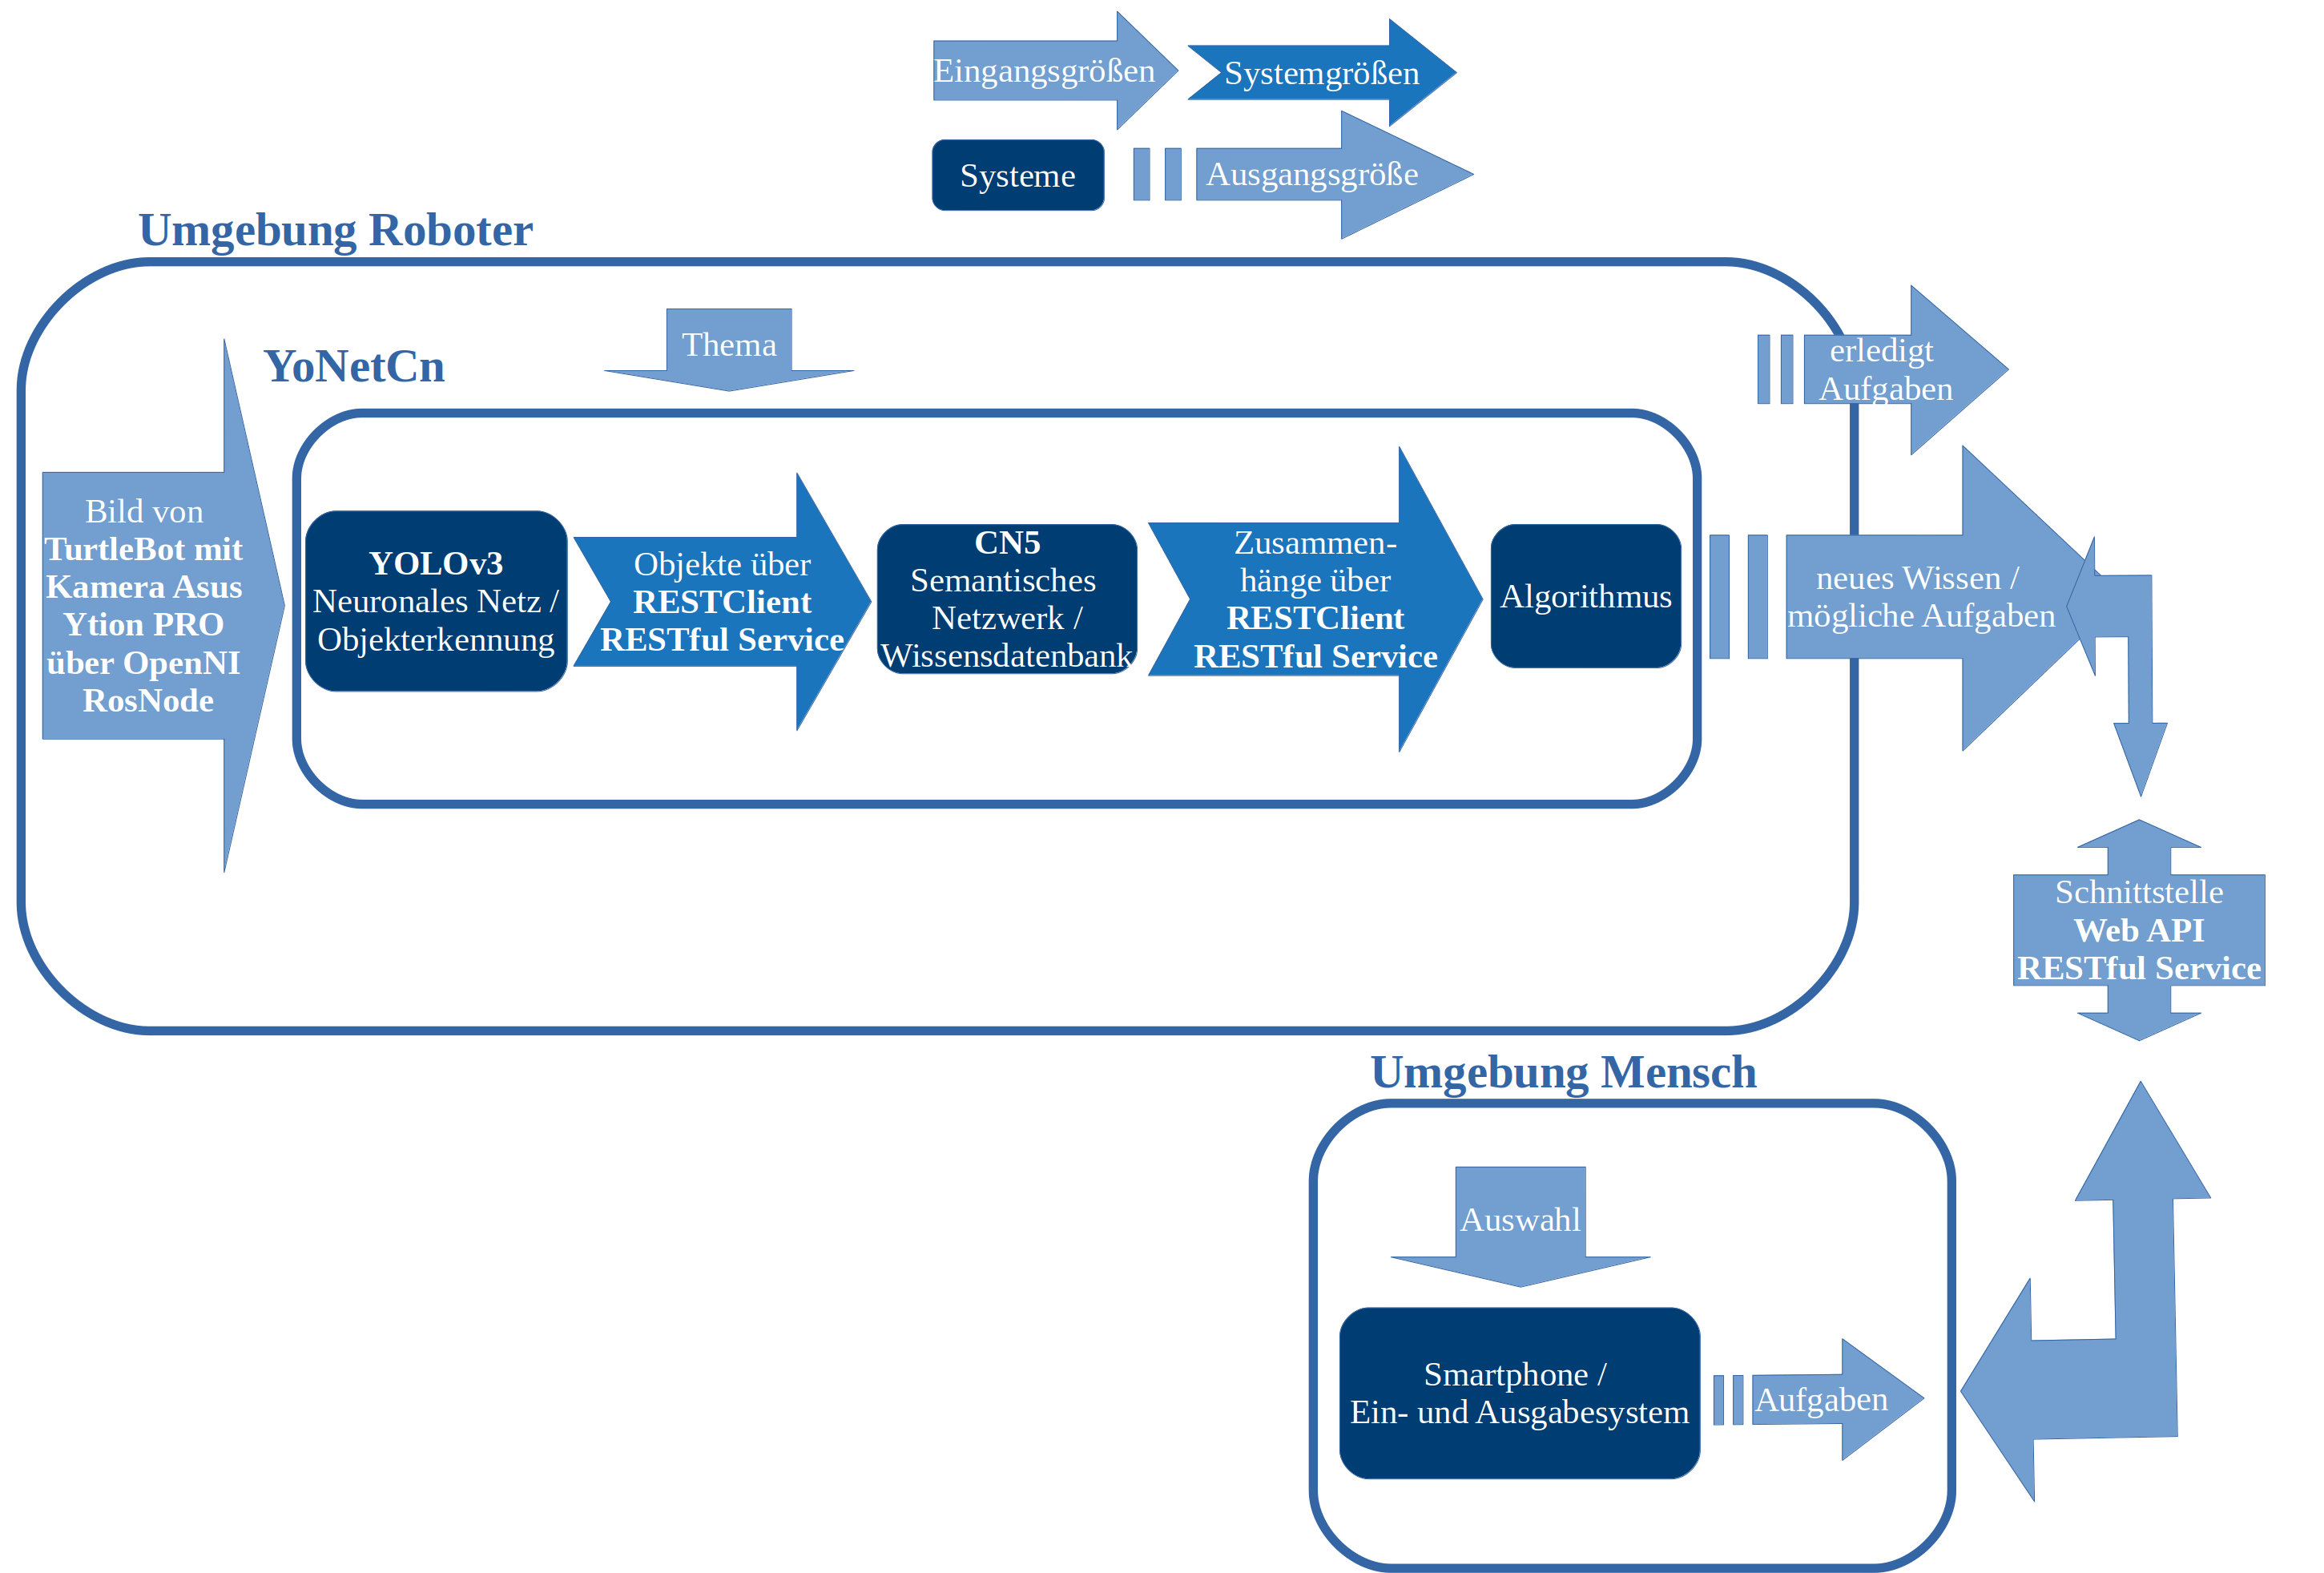
\includegraphics[width=16cm]{images/Masteridee_4.png}
		
		\caption{Roboter Mensch System - erweitert}
		
		\label{Roboter_Mensch_System2}
		
	\end{center}
	
	
\end{figure}

Abbildung \ref{Roboter_Mensch_System2} zeigt das gesamte System mit den in dieser Arbeit umgesetzten Softwarepaketen. 

Objekterkennung

Um YoNetCn nicht nur mit der Asus Kamera zu benutzen, sondern auch Tests mit Bildern anderer Quellen nutzen zu können, wurde eine weitere Eingangsgröße implementiert. Über einen weiteren Ros Publisher können Bilder mit einheitlichem Format nacheinander als Stream in YoNetCn eingegeben werden. Voraussetzung hierbei ist das Bildformat "jpg" und dass alle Bilder die gleiche Breite und Höhe haben. 

Um die Genauigkeit von YoNetCn zu verbessern werden die Namen der erkannten Objekte, die vom Objekterkenner ausgegeben werden, auf Mehrdeutigkeit überprüft und in Richtung Eindeutigkeit angepasst. Die Mehrdeutigkeit der Begriffe können über ein online Wörterbuch en.Wiktionary.org ermittelt werden. Dabei wurde ein Abgleich zwischen deutschsprachigen und englischsprachigen Begriffen vorgenommen. Auffällig dabei ist, dass englische Bergriffe mehr Bedeutungen haben, sich daher die deutsche Sprache grundsätzlich besser für YoNetCn eignen würde. Da jedoch die meisten Objekterkenner und auch Conceptnet primär die englische Sprache nutzen, wurde von einer Übersetzung der Begrifflichkeiten ins Deutsche abgesehen. 

Als besonders kritisch wurde der Begriff mouse eingestuft, da das online Wörterbuch dem Begriff mouse eher das Tier zuordnet, erst als vierte Bedeutung wird hier die Computermaus genannt.
Eine Analyse des COCO Data Set ergab, dass hier keine Bilder vom tierischen Synonym, sondern Bildern von Computer Mäusen hinterlegt sind.
Auf Grund dessen wurde der Begriff mouse in der yolov3.yalm Konfigurationsdatei von "mouse" auf "computer mouse" geändert. 


Eine weitere Unstimmigkeit zwischen den hinterlegten Bildern und dem definierten Begriff des COCO Data Set ist bei dem  "tv" aufgefallen. Dieser ist in der yolov3 Konfiguration bereits standardmäßig auf "tv monitor" umgeschrieben. Da hier nicht nur Bilder von Fernsehern zu erkennen sind, sondern die Bilder eher dem allgemeinerem deutschen Begriff Bildschirm entsprechen, wurde dieser in der Konfiguration von "tv monitor" zu "monitor" geändert. Der Begriff "monitor" ist in so fern kontrovers, da dieser auch die Bedeutung des Überwachers hat und somit keine Eindeutigkeit aufweist. Daher wurden auch die Begriffe "screen" und "display" in Betracht gezogen. Durch das zusätzliche Prüfkriterium, ein Abgleich mit Conceptnet, wurde sich für den Kompromiss "monitor" entschieden. Das ausschlaggebendes Kriterium war die Gewichtung, relatedness, zwischen den Räumlichkeiten und den Begrifflichkeiten. Dabei wurde darauf geachtet, dass die Gewichtung kompatibel bei jenen Räumlichkeiten ist, in denen der Gegenstand zu erwarten ist. 

Der Begriff remote wurde zu remote control, zu deutsch Fernbedienung, geändert. Entsprechend des online Wörterbuches wird remote primär als Adjektiv verstanden und ist im Nominativ nur eine abgekürzte Form von remote contol. Remote ist sicher im englischen Sprachgebrauch eine häufiger zu hörende Form, jedoch wurde hier letztendlich auf Grund des Abgleiches der Gewichtungen von Conceptnet sich für die Begrifflichkeit remote control entschieden.

Laut online Wörterbuch ist der Begriff diningtable ein Tisch, auf dem etwas serviert wird. Die COCO Data Set Bilder zeigen jedoch sämtliche Arten von Tischen. Daher wurden die Begriffe table und desk untersucht. Da desk als Schreibtisch verstanden wird und table eine starke Mehrdeutigkeit aufweist, wurde dieser Begriff nicht abgeändert, ist aber als kritisch zu beurteilen.


Auch der Begriff keyboard wird als kritisch eingeschätzt, da die Bedeutung einerseits als Tastatur, anderseits als Musikinstrument verstanden wird. Weil die primäre Bedeutung sowohl beim online Wörterbuch, als auch beim Abgleich mit den Bildern des COCO Data Set mit dem Begriff der Tastatur übereinstimmen, wurde dieser nicht geändert. 

Auf die Begrifflichkeit der erkannten Objekte wurde besonderer Wert gelegt, da im Laufe des iterativen Entwicklungsprozesses von YoNetCn erkannt wurde, dass die Performance von YoNetCn erheblich von der korrekten und möglichst eindeutigen Beschreibung der erkannten Objekte abhängig ist. 



\begin{figure}[h]
	
	\begin{center}
		
		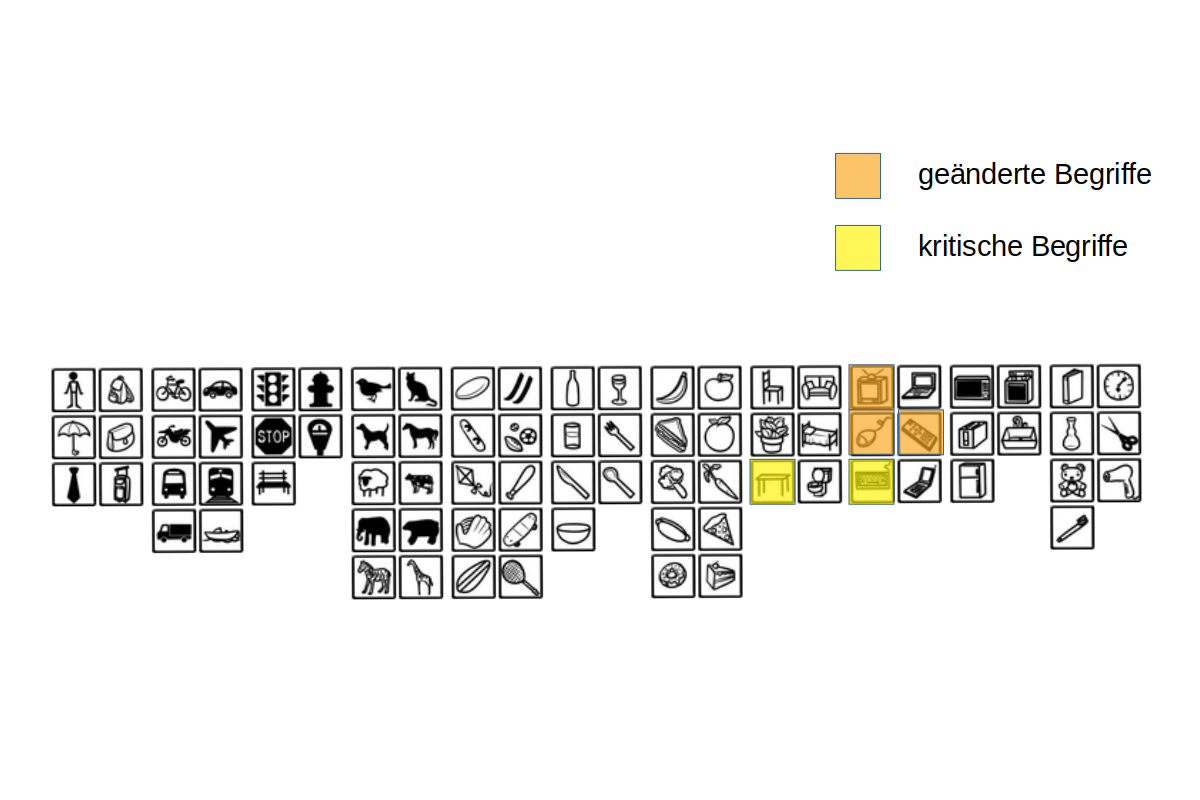
\includegraphics[width=16cm]{images/COCO_Names.png}
		
		\caption{Änderungen der Begrifflichkeiten des COCO Data Set}
		
		\label{COCO_Names}
		
	\end{center}
	
	
\end{figure}

In Abbildung \ref{COCO_Names} sind die Symbole der 80 COCO Data Set Begriffe zu sehen. Die Begriffe der orange markierten Symbole wurden abgeändert, die gelben als kritisch identifiziert.


Die sonstigen Parameter von Yolov3, wie der threshold, die Gewichtungen und die Architektur von Yolov3 wurden nicht geändert. 

Die vom Objekterkenner erkannten Objekte werden in einer zweidimensionalen Matrix zwischengespeichert, wobei die erste Spalte den Namen des Objektes beinhaltet und die zweite Spalte die Häufigkeit des erkannten Objektes. Somit belegen mehrfach erkannte Objekte nicht mehrere Spalten der Matrix. Da diese Matrix zur Abfrage von Conceptnet übergeben wird, resultiert daraus der Vorteil, dass keine Mehrfachabfragen für mehrfach gefundene Objekte stattfinden, wodurch die Bearbeitungszeit deutlich reduziert werden kann. Des weiteren werden in diesem Bearbeitungsschritt Leerzeichen durch Unterstriche ersetzt, da Conceptnet Begriffe die aus mehreren Wörtern bestehen, nur dann verarbeiten kann, wenn diese durch Unterstriche getrennt sind. So wird computer mouse zu computer\_mouse. 


 
 
Wissensdatenbank

Damit die Abfrage des gewünschten Wissens bei Conceptnet erfolgen kann, werden die vom Objekterkenner erkannten Objekte in ein 







\cleartooddpage[\thispagestyle{empty}]
%\cleartoevenpage[\thispagestyle{empty}]

\chapter{Evaluation}
\label{sec:eval}

\section{Evaluation Setup}
\label{sec:evalsetup}


\cleartooddpage[\thispagestyle{empty}]
%\cleartoevenpage[\thispagestyle{empty}]

\chapter{Conclusion}
\label{sec:conclusion}

\section{Summary}
\label{sec:conc:sum}

\section{Future Work}
\label{sec:fw}


\cleartooddpage[\thispagestyle{empty}]
%\cleartoevenpage[\thispagestyle{empty}]

\listoffigures

\lstlistoflistings
%\bibliography{bibtex}

\printbibliography
%\bibliographystyle{apalike}

\end{document}
